\documentclass[twoside,11pt]{article}
%\documentclass[twoside,10pt]{article}

\usepackage{jmlr2e}
\usepackage{spverbatim}
\usepackage{amsmath}
\usepackage{caption}

\newcommand{\ith}{$i^{th}$ }
\newcommand{\jth}{$j^{th}$ }
\newcommand{\weight}{$w_{ji}$ }
\newcommand{\Rw}{\mathbb{R}^w }
\newcommand{\R}{\mathbb{R}}

\begin{document}

\title{Neural Networks Trained by Population Based Algorithms}

\author{\name Andrew Kirby \email andy-kirby@live.com \AND
		\name Kevin Browder \email browderkevin54@gmail.com \AND
		\name Nathan Stouffer \email nathanstouffer1999@gmail.com \AND
		\name Eric Kempf \email erickempf123@gmail.com }

\maketitle

\begin{abstract}

\end{abstract}

\section{Problem Statement}
	% TODO some type of intro about how PBA are considered to be global search methods
	% TODO also mention exploration vs exploitation

	Given data sets, the task is to compare the effectiveness a feed forward Multilayer Perceptron (MLP) trained by Population Based Algorithms (PBA) and Backpropagation. Specifically, there are three PBA: the Genetic Algorithm (GA), Differential Evolution (DE), and Particle Swarm Optimization (PSO). 
	Each training algorithm will be implemented and tested on the following six data sets.
		
	The abalone data set contains features paired with the age of an abalone (the class). The 28 ages are closely related, potentially making classification difficult.
	The car data set contains attributes corresponding to 4 possible conditions of a car while the segmentation data set details 6 distinct subjects of outdoor photographs.
	The rest of the data sets are regression.
	The forest fires set contains the area burned by a forest fire. Most of the values are 0 with a few large values which might give the model trouble.
	The machine data set predicts the performance of a CPU which has an even distribution across its regression values. 
	Wine quality contains the score of a wine with associated attributes. Several of the attributes are correlated, making regression more difficult \citep{datasets}.

\subsection{Hypothesis}

	Population Based Algorithms are expected to outperform Backpropagation because PBA are less prone to getting caught in local minima. 
	Of the PBA, the GA and DE will perform better than PSO because the mutation operator can introduces diversity at any point in a run. 
	
\section{Algorithms}

	Population Based Algorithms typically reference individual members of populations as vectors associated with a fitness value. Each element in a vector corresponds to some value in a model that is being trained by the PBA.
	
	Recall that the output of a Neural Network is entirely dependent on the values of the weights within in the network. 
	So a neural network can be converted to vector form by listing its weights.
	Since weights are real-valued, if $w$ represents the number of weights that a neural network contains then the vector is a point in the Euclidean Space $\mathbb{R}^w$. 
	The fitness associated with the vector is the accuracy or MSE (respectively for classification and regression) of a network on a training data set. 
	
	This sets up the search space of weights and the objective function based on the network's fitness.

\subsection{Genetic Algorithm}

	The Genetic Algorithm (GA) is a evolution-inspired process often used for function optimization. The algorithm represents possible solutions as chromosomes---vectors of genes values that parameterize a model. Given a population of randomly initialized chromosomes, the GA applies cycles of selection, recombination, mutation, and replacement to individuals within the population. Chromosomes with better fitness are expected to survive through these generations, preserving desirable genes as the population searches the fitness landscape \citep{ga_tutorial}.

	At the beginning of a generation, individuals are selected for recombination. Recombination generates an intermediate population by applying crossover between parents, an operator which randomly swaps genes between chromosomes at some rate $P_c$. Next, the mutation operator is applied to each individual in the intermediate population, randomly modifying genes at some rate $P_m$. The intermediate population then completely or partially replaces the original population, completing the generation.
	
	Selecting parents of the intermediate population often follows fitness proportionate selection, rank-based selection, or tournament selection. Fitness proportionate selection selects parents with probability equal to the fitness of the individual divided by the sum of the fitnesses of all individuals in the population. Rank-based selection selects parents with probability
	$$P(\vec{x}_i) = \frac{2}{|P|} \times \frac{|P| - rank(\vec{x}_i)}{|P|+1}$$
	where $|P|$ is the size of the population and $rank(\vec{x}_i)$ is the ranking of the individual $\vec{x}_i$ based on fitness. Ranked-based selection tries to minimize the high selection pressure exhibited by fitness proportionate selection. Another method that balances selection pressure is tournament selection, which selects $k$ individuals from the population at random and chooses the one with the best fitness.

	One-point, two-point, and uniform crossover are common crossover operators. With probability $P_c$, one-point crossover selects a random point in a chromosome, swapping all values of two parent individuals after the crossover point. Two-point crossover swaps values between two selected crossover points. Uniform crossover differs by swapping values at any given point with probability $P_c$. Each crossover operator helps the search by creating children that may inherit more ideal gene combinations from both parents \citep{ga_tutorial}.
	
	%TODO talk about implications of different crossover methods
	
	Mutation operators visit every gene, mutating with probability $P_m$. Specific mutation operators rely on the gene encoding. If genes are binary, mutation flips the bits. If genes are categorical, a new category is chosen from the domain. If genes are real-valued, mutation may generate a new random value or implement creep. With creep, the new gene value $x_i^\prime$ is given by
	$$x_i^\prime = x_i + N(0, \sigma_i)$$
	where $\sigma_i$ is a tunable standard deviation. Mutation helps the search by reinforcing diversity and potentially jumping chromosomes to a completely new spot in the search space \citep{ga_tutorial}.
	
	Replacing the original population with individuals from the intermediate population may follow generational or steady-state replacement. Generational replacement replaces the entire population with the intermediate population. This form of replacement may cause dramatic changes between generations and exhibits a high selection pressure. Steady-state replacement features a more gradual change between each generation by replacing only a proportion of the original population with individuals from the intermediate population.

\subsection{Differential Evolution}
Differential Evolution (DE) is another evolution inspired algorithm with  similarities to GA as both use crossover and mutation on chromosomes. It cycles through selection, mutation, crossover and replacement on individuals in the population.

The DE begins with a population $P$ of vectors that are randomly generated. A target vector $v_t$ is randomly selected from the population. For mutation, a set number of vectors $v_1, v_2,.., v_n$ are randomly selected from the data set. These vectors are combined using the formula below to create a trial vector $v_p$ where $\beta$ is a tuneable parameter. $$v_p = v_1 + \beta(x_2 - x_3) + ... + \beta(x_{n-1} - x_n)$$
Uniform crossover is then applied to the target and trial vector according to a tuning parameter. The fitness for the target and trial vectors are then calculated and if the trial vector has a higher fitness it replaces the target vector. A generation is complete when this process has iterated through the size of the population. 

\subsection{Particle Swarm Optimization}

	PSO differs from the GA and DE in that there is no parent-offspring relationship. Instead, PSO consists of particles that interact and move around the search space to find the optimum solution. 
	
	A swarm consists of $N$ individuals each with a position $\vec{x} \in \Rw$ and a fitness value. 
	PSO then uses an iterative update rule to change each individual's position. The velocity for an individual is named $\vec{v} \in \Rw$, which is composed of 3 summed components.
	
	The first component is inertia. For a given iteration's velocity $\vec{v}_t$, inertia is given as $\omega * \vec{v}_{t-1}$ where $\omega \in \mathbb{R}$ can be referred to as the inertia weight. Note that a ``large inertia weight facilitates a global search while a small inertia weight facilitates a local search" \citep{empirical-pso}.
	
	Second, there is a cognitive component. 
	Each particle records its own best performing position $\vec{x}_c \in \Rw$ across all iterations. 
	With $\vec{x}$ still representing the particle's current position, this component is given as $c_c * r_c * (\vec{x}_c - \vec{x})$ where $r_c$ is randomly selected from $(0,1) \subset \mathbb{R}$ and $c_c$ is a tuned parameter \citep{og-pso}.
	
	The final component is social. 
	For this component, a topology is declared on which particles can communicate between each other.
	Where if two particles $a,b$ can communicate, then $a$ knows both the current position and fitness of $b$.
	Similarly, $b$ knows the current position and fitness of $a$.
	
	Two common topologies used in PSO are the global and local topologies. 
	The global topology allows each particle to communicate with every other particle. 
	The local topology declares that each particle can communicate with only two other particles.
	Specifically, imagine ordering the particles in the order of initialization.
	Then, particle $p_k$ communicates with both $p_{k-1}$ and $p_{k+1}$ where $p_{-1} \equiv p_N$ and $p_{N+1} \equiv p_{0}$.
	This communication persists across all iterations \citep{og-pso}.
	
	Now, take an arbitrary particle $p$ and let $T_p$ denote the set of particles that can communicate with $p$.
	Let $\vec{x}_s \in \Rw$ denote the position of the most fit particle $q \in T_p$. Then, the value of the social component is given as $c_s * r_s * (\vec{x}_s - \vec{x})$ where $r_s$ is randomly selected from $(0,1) \subset \mathbb{R}$ and $c_s$ is a tuned parameter.
	
	Thus the velocity for each particle is given as the sum
	$$\vec{v}_t = \omega * \vec{v}_{t-1} + c_c*r_c*(\vec{x}_c - \vec{x}) + c_s*r_s*(\vec{x}_s - \vec{x})$$
	
	The position of each particle is now updated according to $\vec{x}_t = \vec{x}_{t-1} + \vec{v}_t$. This process is iteratively repeated for each particle until the values of the vectors converge or a maximum number of iterations is reached \citep{og-pso}.
		
\section{Experiment}

\subsection{Evaluation Metrics}

	Classification data sets are evaluated with accuracy and mean squared error (MSE). 
	The MSE metric implemented measures the squared error between the predicted and actual class distributions. 
	This is similar in concept to a Brier score but slightly different in computation. Accuracy indicates how well the algorithm individually classifies examples.
	
	To evaluate regression data sets, mean error (ME) and MSE will be used. MSE squares the distance between a real and predicted value, the squares are then averaged over the entire testing set. 
	ME is computed similarly, but will not square the difference. MSE emphasizes the effect of outliers while ME captures whether the learner tends to over or underestimate the values in the test set. 
	MSE and ME are computed using z-scores (the number of standard deviations from the mean) so that comparisons can be made between data sets.

\subsection{Preprocessing Choices}

	First, all the examples in the data set are randomly scrambled and then assigned to sets for ten-fold cross validation. 
	All categorical variables are converted to integers 
	and the preprocessor also generates a similarity matrix for each categorical variable that is used for determining distances between categorical variables. 
	All numerical variables are normalized between 0 and 1. 
	The data sets did not contain any missing variables.

\subsection{Algorithm Choices}

\subsubsection{Genetic Algorithm}

	Any GA implementation requires specific crossover, mutation, selection, and replacement methods. For this implementation, uniform crossover, creep mutation, rank-based selection, and steady-state replacement. Uniform crossover was selected for its more disruptive tendencies, a desirable trait for low population implementations \citep{ga_tutorial}. Creep mutation was selected for its stability. Rank-based selection is expected to provide practical convergence times while supporting diversity in the population. A bonus is that this method mitigates the large decrease in selective pressure as the members of the population approach similar fitnesses \citep{ga_tutorial}. Additionally, rank-based selection had no tunable parameters. Steady-state replacement was implemented by generating an intermediate population one fourth of the size of the original population. Then, intermediate population members replaced random members in the original population, but only if they had better fitness.	

\subsubsection{Differential Evolution}

\subsubsection{Particle Swarm Optimization}

	% TODO write the choices/reasoning we made to avoid tuning, this should be done for each algorithm
	
	Two decisions were made for PSO. First, the global topology was declared on how particles in the swarm communicate. 
	The global topology is the original topology used in PSO and was chosen over the local topology because it has been reported that the local topology requires more iterations to reach a specified error level \citep{og-pso}. 
	Second, the $\omega$ term in the velocity equation decreases linearly over the course of a run. Experimentally, a linearly decreasing $\omega$ from 0.9 to 0.4 provides a nice exploration-exploitation balance for PSO \citep{inertia}.

\subsection{Tuning}

\subsubsection{Genetic Algorithm}

\subsubsection{Differential Evolution}

	Tuning for DE requires tuning the crossover($P_c$) and mutation ($\beta$) parameters. A grid search was performed between $P_c$ and $\beta$ on each dataset with $P_c \in \{.25, .5, .75\}$ and $\beta \in \{.5, 1, 1.5\}$.
	The optimum values were then selected for each dataset based on the results from this search. 

\subsubsection{Particle Swarm Optimization}	

	Tuning for PSO requires setting the values of $c_c$ of $c_s$. 
	Experimentally, PSO performs best with $c_c = c_s = 2$ \citep{empirical-pso}. 
	As such, a grid search was performed on $ (c_c, c_s) \in \{ 1, 2, 3 \} \times \{ 1, 2, 3 \} $ for each data set. 
	Then the optimum parameters were selected based on fitness of the produced networks (accuracy for classification and MSE for regression).
	In general, the classification data sets performed best with $c_c > c_s$ while the regression data sets preferred $c_c < c_s$.

\section{Results}

	For the final run, optimal parameters were selected for each data set. In general, Backpropagation outperformed the PBA on classification data sets while the opposite is true for regression data sets. This partially realized the hypothesis that Population Based Algorithms would perform better than Backpropagation.

	\begin{figure}[h]
		\centering
		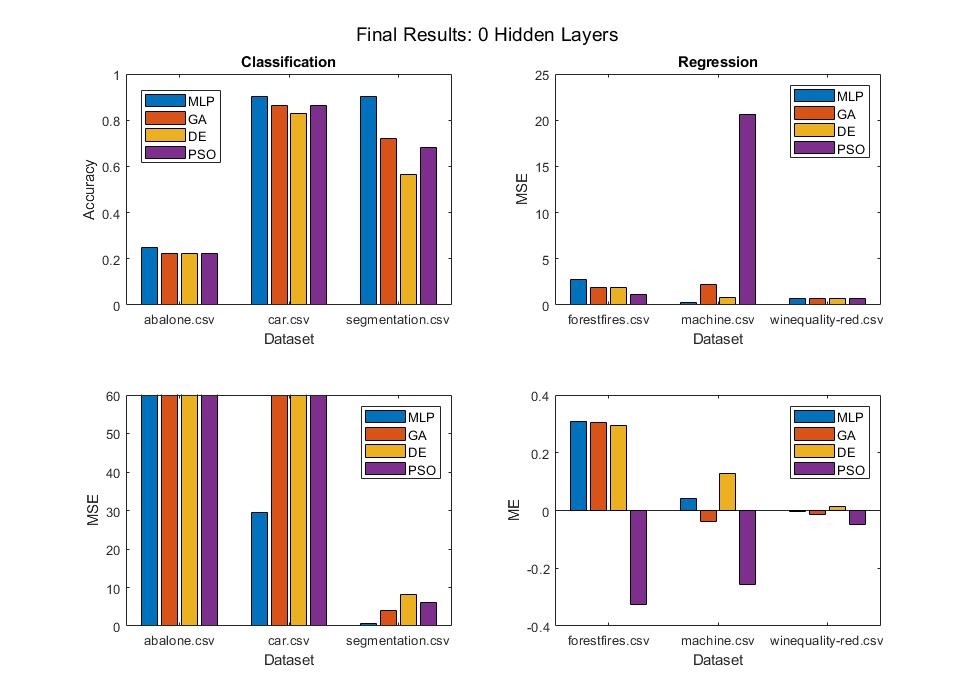
\includegraphics[height=3in]{FINAL_FIGS/0_hl.jpg}
		\caption{Final Results of a 0 Hidden Layer MLP. Color indicates training algorithm type.}
		\label{0-hl}
	\end{figure}
	
	\begin{figure}[h]
		\centering
		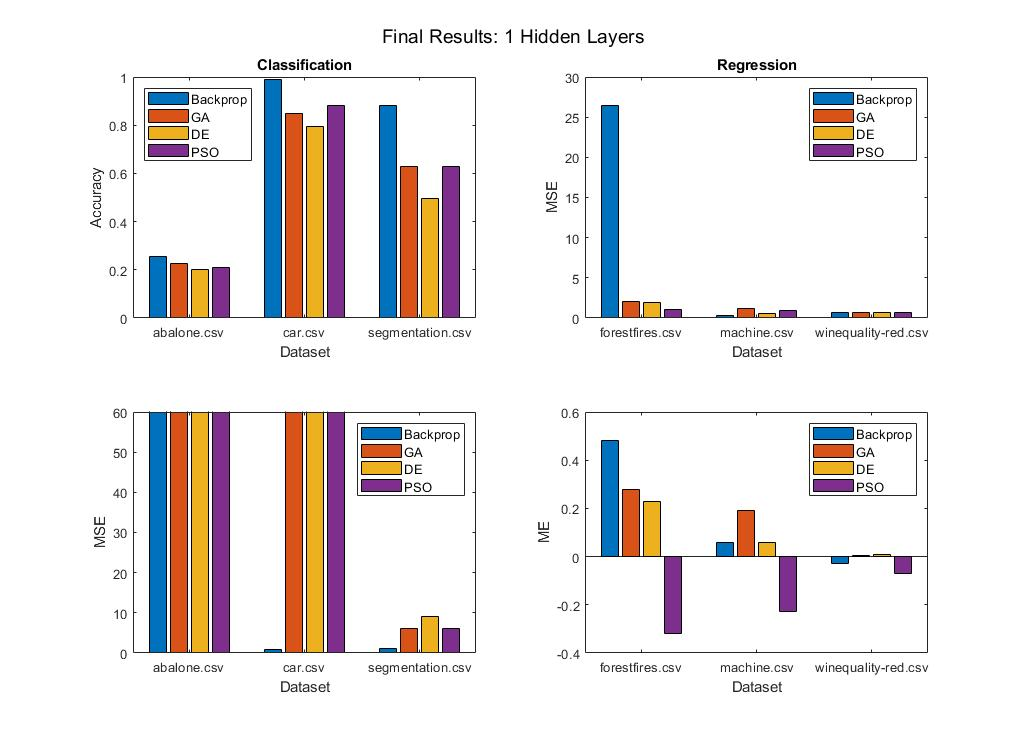
\includegraphics[height=3in]{FINAL_FIGS/1_hl.jpg}
		\caption{Final Results of a 1 Hidden Layer MLP. Color indicates training algorithm type.}
		\label{1-hl}
	\end{figure}
	
	\begin{figure}[h]
		\centering
		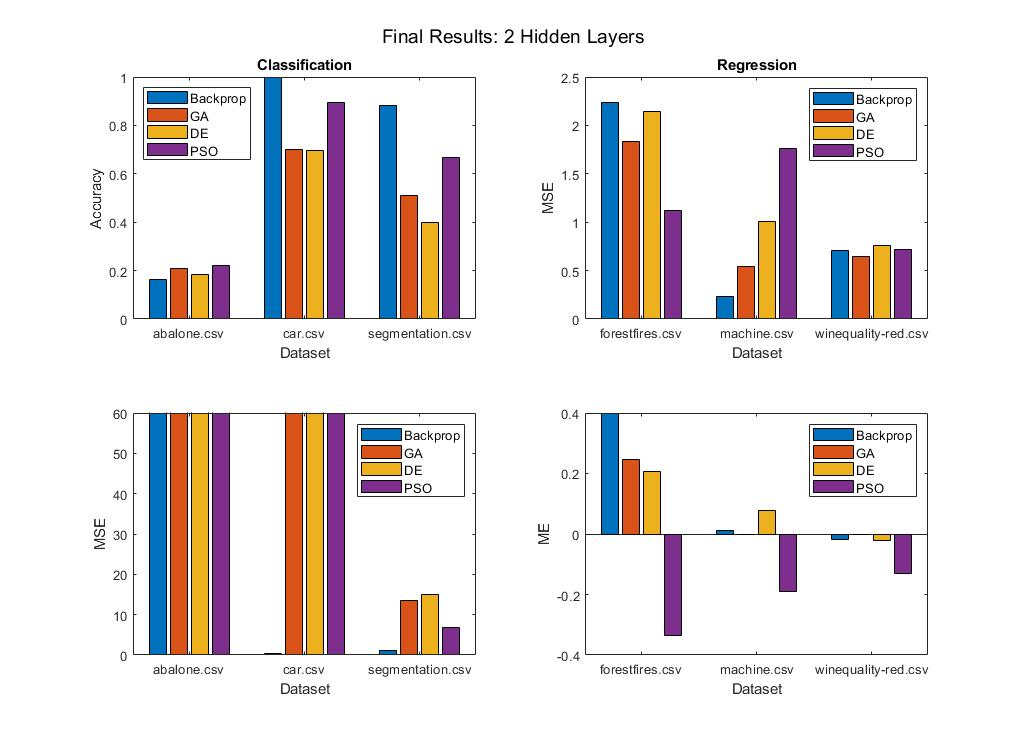
\includegraphics[height=3in]{FINAL_FIGS/2_hl.jpg}
		\caption{Final Results of a 2 Hidden Layer MLP. Color indicates training algorithm type.}
		\label{2-hl}
	\end{figure}

	The greatest difference in performances between the two algorithms is shown on the forest fires data set in Fig. \ref{1-hl} where the MLP has 1 hidden layer. 
	For a network trained with Backpropagation, the MSE was 26 while the MSE for networks trained with PBA is less than 3. 
	The most likely explanation is that the PBA were able to pass by the local optima that Backpropagation found for the configuration of weights.

\section{Summary}

\newpage

\bibliography{biblio}

\end{document}
